\documentclass[handout]{beamer}
\usepackage{multicol}
\everymath{\displaystyle}
\mode<presentation>
{\usetheme{Warsaw}\setbeamercovered{dynamic}}
\usecolortheme{crane}
\usepackage{beamerfoils}
\pgfdeclareimage[height=1in]{university-logo}{ISULogo}
\logo{\pgfuseimage{university-logo}}
\setbeamertemplate{navigation symbols}{}
\title[Roulette]{Roulette}
\author{Dr Marcus Bishop}
\subject{Math 104}
\beamerdefaultoverlayspecification{<+->}
\theoremstyle{definition}
\newtheorem{remark}{Remark}
\newtheorem{impact}{Impact}
\newtheorem{notation}{Notation}
\usepackage{arev}
\begin{document}
\begin{frame}\titlepage\end{frame}
\LogoOff
\begin{frame}{Roulette}
\begin{multicols}{2}
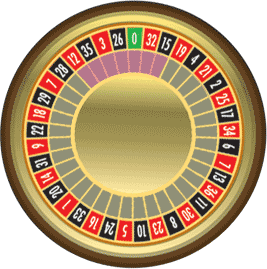
\includegraphics[scale=.38]{Roulette}
\begin{itemize}
\item Roulette wheel has slots numbered $1$--$36$
\columnbreak
\item American wheel also has slots $0$ and $00$
\item $18$~slots red, $18$~slots black, $0,00$ green
\item Can bet that ball stops on particular number
\item Bet called \alert{straight up}
\item If ball stops on that number, casino pays player
$35$ times bet
\item If not, casino keeps bet
\end{itemize}
\end{multicols}
\end{frame}

\begin{frame}{Straight up}
\begin{itemize}
\item Calculate expected proceeds from betting $\$1$
on a particular number, a \alert{straight up}
\item Wheel has $38$ spaces, each equally likely
\item So $\frac{1}{38}$ the probability of winning
\item $\frac{37}{38}$ the probability of losing
\item $35\left(\frac{1}{38}\right)
+\left(-1\right)\left(\frac{37}{38}\right)
\only<+->{=\frac{35-37}{38}}
\only<+->{=-\frac{2}{38}}
\only<+->{=-\frac{1}{19}}$
\item Thus $-\frac{1}{19}\approx -0.053$ the expected proceeds
\end{itemize}
\end{frame}

\begin{frame}{Street}
\begin{itemize}
\item Can also bet on three numbers
\item Bet called a \alert{street}
\item (Numbers must lie in same row of \alert{layout})
\item If ball stops on any of those numbers, casino
pays player $11$ times bet
\item Calculate expected proceeds from betting $\$1$ on a street
\item $11\left(\frac{3}{38}\right)+\left(-1\right)\left(\frac{35}{38}\right)
\only<+->{=-\frac{2}{38}}
\only<+->{\approx -0.053}$
\end{itemize}
\end{frame}

\begin{frame}{Rule for roulette payouts} 
\begin{itemize}
\item In general, players can bet on $n$
chosen numbers for any $n$
\item (Chosen numbers subject to arrangement of layout)
\item Casino pays $\frac{36}{n}-1$ times
bet if ball lands on one of chosen numbers
\item For example,
\[\begin{array}{l|c|l}
n&\frac{36}{n}-1&\text{Name}\\\hline
1&35&\text{straight up}\\
3&11&\text{street}\\
18&1&\text{red, black, even, odd}
\end{array}\]
\end{itemize}
\end{frame}

\begin{frame}
\begin{itemize}
\item If $0$ and $00$ were removed, would be $36$ rather than $38$ spaces
\item So $\frac{1}{36}$ the probability that ball stops on particular number
\item If bet contains $n$ numbers
\[\left(\frac{36}{n}-1\right)\frac{n}{36}
+\left(-1\right)\frac{36-n}{36}
\only<+->{=1-\frac{n}{36}-1+\frac{n}{36}}
\only<+->{=0}\]
\item Thus roulette would be fair, if not for extra spaces $0$ and $00$!
\item In long run, players would win nothing and casino would not profit
\end{itemize}
\end{frame}
\end{document}
